\documentclass[10pt,a4paper]{article}
\usepackage[utf8]{inputenc}
\usepackage[english]{babel}
\usepackage{amsmath}
\usepackage{amsfonts}
\usepackage{amssymb}
\usepackage{graphicx,float}
\usepackage{subcaption}
\usepackage{float}
\begin{document}
\author{\textbf{Onuray SANCAR}}
\title{\textbf{Experiment 1, The Stefan-Boltzman Radiation Law}}
\date{November 22, 2019}
\maketitle
\textit{with} {\large\textbf{{Yaren AKSEL}}\textit{,} \textbf{Experiment Date}:Novermber 15, 2019\\[3\baselineskip]
\textbf{Abstract}\\[\baselineskip]
\par The purpose of our experiment is to observe some applications of lasers: We have calculated a distance using laser and our values was $3\sigma$ away from the measured values. We have measured the wavelength of our light using grating and found the wavelength as $\lambda=(5.5\pm3.7)\times100$nm which was 0.22$\sigma$ away from the given value. We have measured the diameter of a hair and the value we get is a plasusible diameter for a human hair. We have measured the index of refraction of a tranparent solid using the michelson interferometer and we have found index of refraction as $n=1.09\pm0.14$.
\begin{figure}[H]
	\begin{center}
		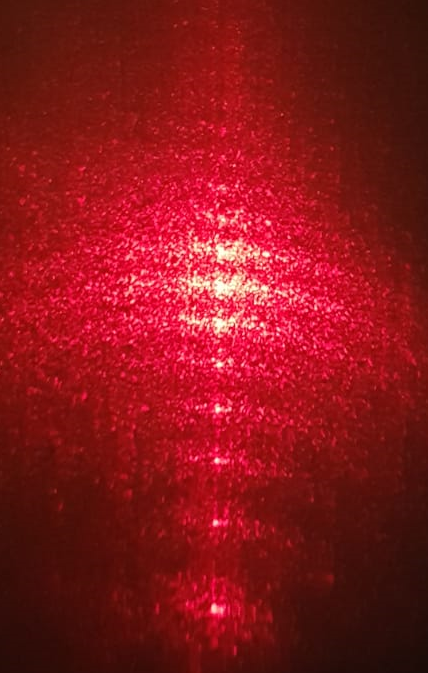
\includegraphics[scale=0.5]{doubleslit.png}
	\end{center}
\end{figure}
\textbf{Theory}\\[\baselineskip]


\textbf{\small{Triangulation}}
\par Triangulation is a really old technique and it has a rather broad usage from calculating distances between stars to measuring small lengths precisely in labs. We use lasers for our triangulation. A sketch for easiness is given:
\begin{figure}[H]
	\begin{center}
		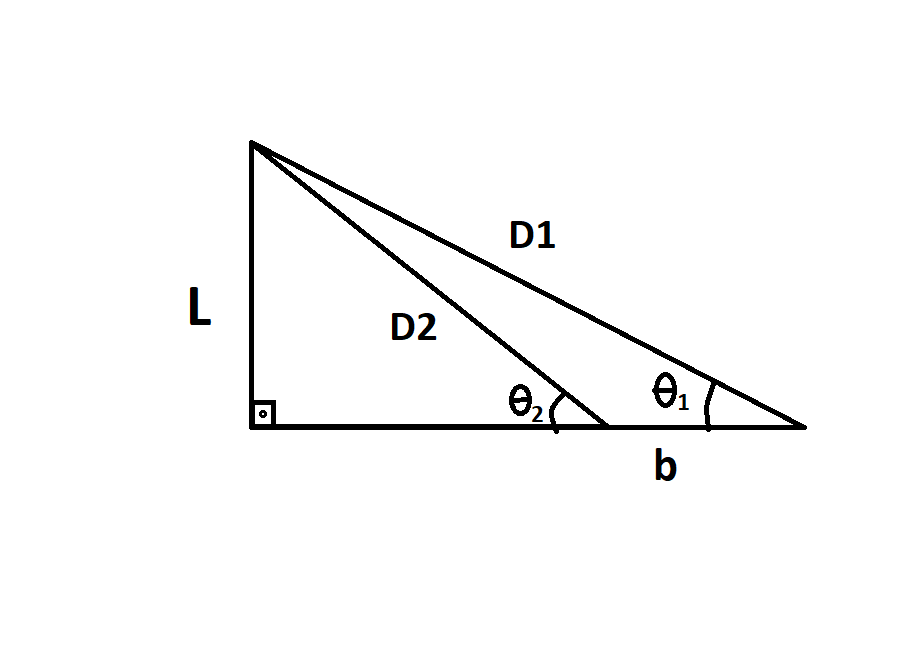
\includegraphics[scale=0.6]{d1d2.png}
	\end{center}
\end{figure}
\par We point a laser from a baseline to some point with an angle $\theta_1$ and $\theta_2$ with distance from that points being $D_1$ and $D_2$ respectively. The distance between the lasers at the baseline is b and the distance from the baseline to the point lasers point at is L. 
\par To find L, first we see that
\par $D_2.sin\theta_2=D_1.sin\theta_1=L$
\par Also $D_2.cos(\theta_2)+b=D_1.cos\theta_1$
\par Then plugging $D_2=D_1.sin\theta_1/sin\theta_2$ to the previous equation we get
\par $b=D_1(cos\theta_1.sin\theta_2-sin\theta_1cos(\theta_2))/sin\theta_2$
\par Then $D_1=b\times sin\theta_2/sin(\theta_2-\theta_1)=b\times sin(\pi-\theta_2)/sin(\theta_2-\theta_1)$
\par Plugging this to the $D_2.sin\theta_2=D_1.sin\theta_1$:
\par $D_2=b\times sin\theta_1/sin(\theta_2-\theta_1)$
\par Taking $D_2.sin\theta_2=D_1.sin\theta_1=L$ into account we can find L.
\textbf{\small{Finding Wavelength}}
	\par We used a ruler with spacing d for reflecting grating purposes. A reflecting grating with widely speced grooves gives good diffraction spectra if the incedent light is nearly parallel to the surface of the grating.$^1$ Let's derive the formula for the wavelength.
\begin{figure}[H]
	\begin{center}
		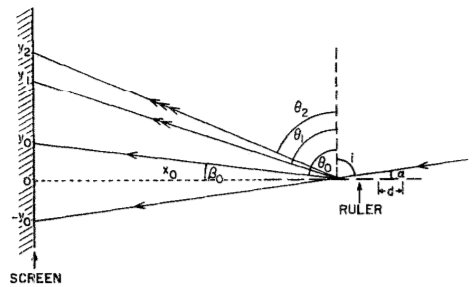
\includegraphics[scale=0.9]{cetvel.png}
	\end{center}
\end{figure}
As we see from the figure we can write the grating equation as
\begin{equation}
n\lambda=d(sini-sin\theta)
\end{equation}
where n is an integer, $\lambda$ is the wavelength, and d is the spacing between rulings. It is more convenient to write $\alpha=90^o-i, \beta=90^o-\theta$ then the equation becomes$^1$
\begin{equation}
n\lambda=d(cos\alpha-cos\beta)
\end{equation}
Also, $\alpha=\beta_0$ and $tan\beta=y_n/x_0$ because $\beta$ is small, so that $tan\beta\approx sin\beta$.
\begin{figure}[H]
	\begin{center}
		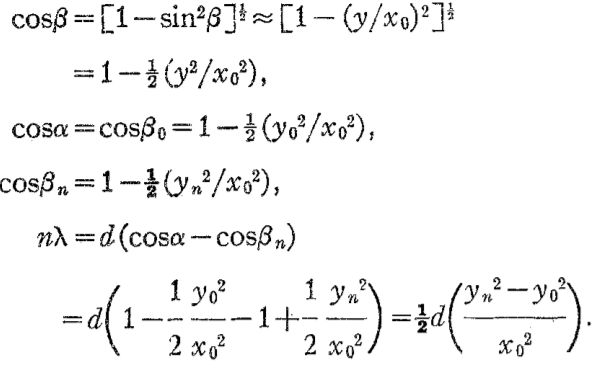
\includegraphics[scale=0.7]{cet.png}
	\end{center}
\end{figure}
\textbf{\small{Measuring the diameter of hair}}
\par When light passes through a single slit whose width w is on the order of the wavelength of the light, then we can observe a single slit diffraction pattern on a screen that is a distance L >> w away from the slit.  The intensity is a function of angle.  Huygens' principle tells us that each part of the slit can be thought of as an emitter of waves.  All these waves interfere to produce the diffraction pattern.  Where crest meets crest we have constructive interference and where crest meets trough we have destructive interference.$^4$
\par By shining a laser at an hair, we are in a sense creating infinetly many small slits with total length of d thanks to the empty spaces between molecules. This is a way to obtaing single slit from many slits. We can accept this idealization because the diamter is huge compared to the molecular distances.
\par Then using one slit equation $dsin\theta_n=n.\lambda$ where n=1,2,3,... we can calculate the diameter of hair d by looking at angles from the horziontal line where we put our hair.
\\[\baselineskip]
\textbf{\small{Measuring the index of refraction of a transparent solid}}
\par Light, since it has different speeds at different mediums, causes phases difference in different mediums when the same distance is traveled. This phase difference/path difference is related to the index of refraction of the material. So finding the index of refraction of some material by using these phases differences is what we are trying to achieve. The optical path differences can be measured very accurately with the help of a Michelson's interferometer.$^2$
\par Assume that we have a transparent solid object whose thickness is d and its index of refraction is n. For normal incidence of light rays, the optical path length is simply
\par$L_{perpendicular}=n.d+\frac{d}{cos\theta_i}-d$
\par Rotating the solid like the figure given below around its vertical axis
\begin{figure}[H]
	\begin{center}
		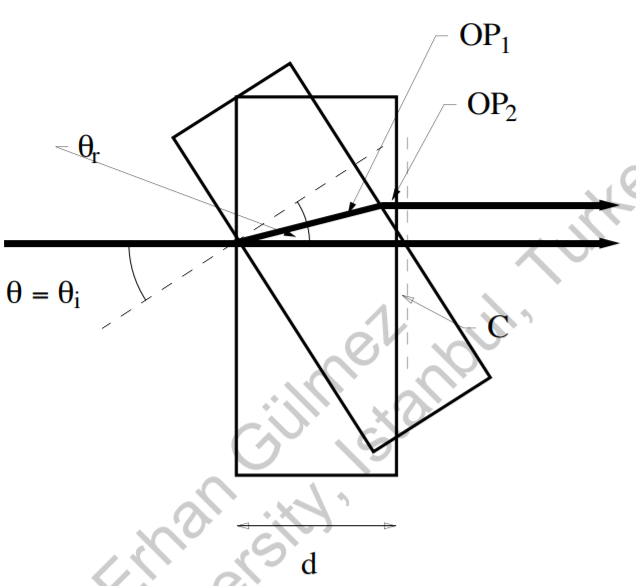
\includegraphics[scale=0.6]{n.png}
	\end{center}
\end{figure}
We can determine the angle of refraction inside the solid from the Snell's law($n_{air}=1$)$^2$
\begin{equation}
\frac{sin\theta_i}{sin\theta_r}=n.
\end{equation}
\par When the solid is rotated we get
\begin{equation}
OP_1=\frac{nd}{cos\theta_r}
\end{equation}
To find $OP_2$ we first project $OP_1$ to the horizontal line which is $OP_1\times cos(\theta_i-\theta_r)$ and we subtract this projection from the unturned distance nd:
\begin{equation}
OP_2=nd-\frac {nd}{cos\theta_r}cos(\theta_i-\theta_r)=
\end{equation}
\begin{equation}
OP_2=\frac{d}{cos\theta_r}sin(\theta_i-\theta_r)tan(\theta_i)
\end{equation}
Then, the total optical path length when the transparent solid is at an angle $\theta$ with respect to the incident beam is$^2$
\begin{equation}
L_{theta}=OP_1+OP_2=\frac {nd}{cos\theta_r}(1+\frac {sin(\theta_i-\theta_r)tan\theta_i}{n}).
\end{equation}
Net path difference is then
\begin{equation}
\Delta L= L_{\theta}- L_{perpendicular}	
\end{equation}
By the phase difference caused by the michelson interferometer, we will observe 'movement' of fringes. The number m of fringes moved will be $^2$
\begin{equation}
m=\frac {2\Delta L}{\lambda}
\end{equation}
By leaving the index of refraction alone we get:
\begin{equation}
n=\frac {(d-m\lambda/2)(1-cos\theta_i)}{d(1-cos\theta_i)-m\lambda/2}
\end{equation}
\textbf{Apparatus}\\[\baselineskip]

\begin{itemize}
	\item \textbf{Low Power He-Ne Laser}: Laser used in the experiment. It produces light with 633nm.
	\item \textbf{Ruler}: Used to measure distances.
	\item \textbf{Protractor}: Used to measure angle that the laser make with the baseline in the first part.
	\item \textbf{Metal Ruler}: Used in the grating part as the grating.
	\item \textbf{Hair}: Used to measure the diameter of hair by acting like a one slit.
	\item \textbf{Michelson's Interferometer}: Used to create phase difference between the lights from two differents arms to see fringes on some distant screen
	\item \textbf{A Transparent Solid Sample}: We are trying to measure its index of refraction.
	\\[\baselineskip]
\end{itemize}
\textbf{Procedure}\\[\baselineskip]
\begin{enumerate}
	\item We have closed the lights so we can see the effects of light easier.
	\item 1st part.We have chosen a baseline some distance away from the screen/wall parallel to the wall. We have put laser at an angle $\theta_1$ with the baseline, pointing at some chosen point on the screen. Then we have chosen another angle $\theta_2$ distance b away on the baseline from the fisrt point we have put our laser, so that the laser is still pointing at the previously chosen point at the screen. We have measured the dşstance from the baseline to the screen for later comparison.
	\item 2nd part. We have point our laser to a metal ruler's spacings with an angle so that we can see a grating pattern on the screen. The spacing between the ruler is d, the ruler is put distance x away from the screen. We have alligned the ruler and laser such that they were on the same line. The diffraction pattern is observed and the maxima points are measured with respect the vertical distance from the ruler.
    \item 3rd part. We have put a hair piece horizontal to the ground at some object and shine the laser on the hair, we have seen the one slit pattern on the screen. The distance between the hair and the screen is again x. We have measured the minima positions with respect to some chosen origin.
    \item 4th part. First we have have calibrated the interferometer such that the phase difference was eliminated. Then we have put our transparent solid in one arm of the Michelson interferometer and using an arm near it we have rotated this transparent solid at regular intervals. We have recorded the number of fringes past from a distant screen at these regular intervals.
\end{enumerate}
\textbf{Data}\\[\baselineskip]
\par The Triangulation part:
\begin{figure}[H]
	\begin{center}
		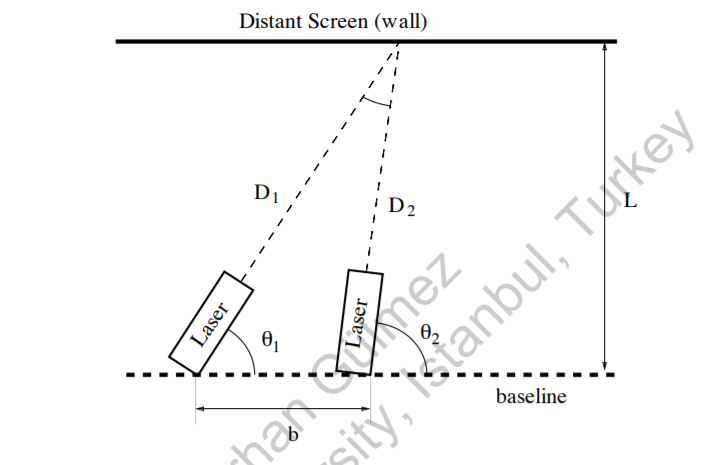
\includegraphics[scale=0.75]{Tri.png}
	\end{center}
\end{figure}
\par b=$13.80\pm0.05$cm, $L=104.2\pm0.1cm$, $\theta_1=73\pm1^o$ and$\theta_2=80\pm1^o$.
\begin{center}
\begin{figure} [H] 
\begin{tabular}{|c |c|} \hline
$y_n$& y distance from the horizontal line of the Ruler(cm) \\ [0.5ex] 
\hline
y0&3.8 \\
\hline
y1 & 6.7\\
\hline 
y2 &8.8\\
\hline 
y3& 10.5 \\
\hline 
y4 & 12.0\\
\hline 
y5 &13.4\\
\hline 
y6 & 14.7\\
\hline
y7&15.9\\
\hline		
\end{tabular}
		\caption{Data for finding the $\lambda$ part of the experiment.The distance between the screen and the ruler is $x=121.3\pm0.8$cm, spacing between the ruler is d=0.05cm and it is taken as given.Errors of the $y_n$s' are the same and the value are 0.1cm.}
	\end{figure}
\end{center}
\begin{center}
	\begin{figure} [H] 
		\begin{tabular}{|c |c|} \hline
			Minima points $y_n$& Vertical distance from the desk \\ [0.5ex] 
			\hline
			$y_{-9}$&6.5 \\
			\hline
			$y_{-8}$ & 7.3\\
			\hline 
		$y_{-7}$ &8.0\\
			\hline 
			$y_{-6}$& 8.7 \\
			\hline 
		$y_{-5}$ & 9.4 \\
			\hline 
			$y_{-4}$ &10.1\\
			\hline 
		$y_{-3}$ & 10.8\\
			\hline
			$y_{-2}$&11.5\\
			\hline
			$y_{-1}$&12.1 \\
			\hline
			$y_{1}$ &13.5\\
			\hline 
			$y_{2}$ &14.1\\
			\hline 
		$y_{3}$& 14.9 \\
			\hline 
			$y_{4}$ & 15.5\\
			\hline 
		$y_{5}$ &16.2\\
			\hline 
			$y_{6}$ & 17.0\\
			\hline
			$y_{7}$&17.6\\
			\hline	
			$y_{8}$ & 18.3\\
			\hline
			$y_{9}$&18.9\\
			\hline		
		\end{tabular}
		\caption{Data for finding the diameter of a hair part of the experiment.The distance between the screen and the laser is $x=126.0\pm0.1$cm and the origin is taken as $12.8\pm0.1$ cm. Errors of the $y_n$s' are the same and the value are 0.1cm.}
	\end{figure}
\end{center}
\begin{center}
	\begin{figure} [H] 
		\begin{tabular}{|c |c|} \hline
			Number Read on the Turning 'Ruler' (units)& Number of Fringes Past \\ [0.5ex] 
			\hline
			0.25&0 \\
			\hline
			0.50 & 2\\
			\hline 
			0.75 &5\\
			\hline 
			1.00&8 \\
			\hline 
			1.25 &8 \\
			\hline 
			1.50 &13\\
			\hline 
			1.75 & 15\\
			\hline
			2.00&18\\
			\hline
			2.25&23 \\
			\hline
			2.50 &23\\
			\hline 
			2.75 &25\\
			\hline 
			3.00&27\\
			\hline 
			3.25 & 29\\
			\hline 	
		\end{tabular}
		\caption{Data for finding the index of refraction of a transparent solid part of the experiment.The width of the solid is taken as 0.60cm, there is no uncertainty assigned to this value because we did not measure it. Errors of the 'ruler' values are the same and the value are 0.05units. 4 units this 'ruler' correspond to $1.00\pm0.01$cm of horizontal difference.Distance from the center of rotation to one of the ends is 3.1cm, we take this as given as well because we forgot to measure it.}
	\end{figure}
\end{center}
\textbf{Analysis}\\[\baselineskip]
\textbf{\small{Some Useful Formulas}}
\par Error propagation
\begin{equation}
{\sigma }_{f}=\sqrt{\sum _{i}^{n}{\left(\frac{\partial f}{\partial {x}_{i}}\right)}^{2}{\sigma }_{{x}_{i}}^{2}+\dots }
\end{equation}
\par Weighted average
\begin{equation}
f_{weighted}=\frac{\sum _{i}\frac{{f}_{i}}{{\sigma_i }^{2}}}{\sum _{i}\frac{1}{{\sigma_i }^{2}}}
\end{equation}
\par Where $\sigma_i$ is the uncertainty in $f_i$
\\[\baselineskip]
\textbf{\small{Triangulation}}
\begin{figure}[H]
	\begin{center}
		\includegraphics[scale=0.8]{tri.png}
	\end{center}
\end{figure}
\par Using the equations we have derived for $D_1$ and $D_2$ we get:
\par $D_1=111.5\pm 0.8 cm$ and $D_2=108.3cm\pm0.7$
\par By taking sine of these values respectively to their angles, we get L:
\par $L_1=106.6cm \pm0.8$cm and $L_2=106.6cm\pm0.8$cm
\par The value we found for the length is $L=106.6cm \pm0.8$cm and it is 3.0$\sigma$ away from the value we have measured.
\\[\baselineskip]
\textbf{\small{Finding the Wavelength}}
\par Since the equation is described as:
\begin{figure}[H]
	\begin{center}
		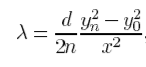
\includegraphics[scale=0.8]{lambda.png}
	\end{center}
\end{figure}
\par We plug our datas to the formula above, obtaining 7 different $\lambda$ values. Since they are all measured with the same apparatus, they have the same uncertainty, so taking the weighted mean is really easy and we get $\lambda_{weighted}=5.5\times 10^{-5}$cm. To calculate the error of the wavelength, we use error propagation formula above and obtain $\lambda_{error}=3.7\times 10^{-5}$cm.
\par Then the wavelength is  $\lambda=(5.5\pm3.7)\times 10^{-5}$cm or $\lambda=(5.5\pm3.7)\times100$nm. Which is 0.22$\sigma$ away from the given 633nm wavelength of the laser.
\\[\baselineskip]
\textbf{\small{Finding the Diameter of Hair}}
\par We know n,x and $\lambda$ in the minima equation $d\mathrm{sin}{\theta }_{n}=n\lambda$. Then by finding $\theta_n$ we can obtain the dimater of the hair, d.
\par First, we subtract the so called origin from the $y_n$ values for ease of doing our calculations. The error of each distance then becomes 0.14 cm which with consideration of significant figures downgrades to 0.1 cm.
\begin{figure}[H]
	\begin{center}
		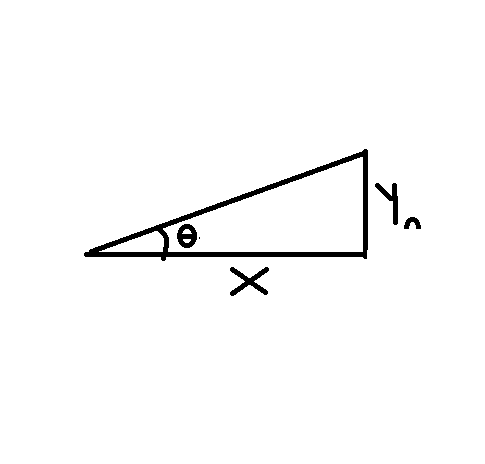
\includegraphics[scale=0.6]{Arctan.png}
	\end{center}
\end{figure}
\par By taking the arctan of the $y_n/x$ values, we can obtain $\theta_n$ values. After obtaining these values we put them into the minima equation and get 18 d values. By taking weighted average of them using the weighted average formula above in conjunction with the minima equation we get: d=0.010cm
\par To calculate the uncertainty of d we use the error propagation formula in conjunction with the minima equation: $d_{error}=0.001$cm.
\par Diameter of the hair we experimented on is then found as $d=0.010\pm0.001$cm or $d=(1.0\pm0.1)\times 100\mu m$. Average hair diameter is between $15\mu m$ and $180\mu m$ so our calculation sits within this range.
\\[\baselineskip]
\textbf{\small{Finding the Index of Refraction of a Transparent Solid}}
\par Using the equation we have derived in theory part, we plug the d, m, $\lambda$ values directly to the equation:
\begin{figure}[H]
	\begin{center}
		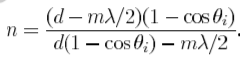
\includegraphics[scale=0.8]{index.png}
	\end{center}
\end{figure}
\par To find $\theta$, we convert the turning units to cm by dividing them with 4 (using the fact that 4 units correspond to 1cm) and then by using the same technique as the previous analysis part we find $\theta$ values. Then we plug now known $\theta$ values to the above equation and get various index of refractions. By taking the weighted average of these by using the weighted average formula in conjunction with the formula for index of refraction we get $n=1.09$
\par Also by using the error propagation formula we find the uncertainty of n as 0.14.
\par The index of refraction is $n=1.09\pm0.14$.
\\[\baselineskip]
\textbf{Conclusion}\\[\baselineskip]
We have looked at some of the applications of lasers. For the triangulation part, the value we have found is 3$\sigma$ away from the value we have measured independently. We were expecting a rather precise value but we were quite off. There are several possible reasons for this: first, we might not have measured the distance correctly after all the distance is rahter large and we could have shifted the ruler. Second, we might have measured the distance b incorrectly. Third and the most likely reason is that we might not have pointed the lasers at the same location, the light was casting a rather big image and we were kind of blinded by its intensity.By introducing more rigid apparatus that can be moved on trails instead of using ruler and pen we could have solved many possible problems.
\par For finding the wavelength part, our values was 0.22$\sigma$ away from the given value of the wavelength, We have observed slits rather beautifully on the screen, that is why we have put the image of slits(it looks much better in person)!. Only thing that might have cast a shadow (pun intended) on the experiment is allignment of the ruler and laser. We have put whatever we can hold below the laser and ruler to allign them well. This could have caused some issues. 
\par For finding the hair diameter part, our value accuratetly represents a human hair. But the thing is human hair is not in single size and the variation of size from human to human varies drastically. Although our value seems good, there was no way of knowing whether it has substantial error or not.
\par For finding the index of refraction part, we have found the index of refraction as $n=1.09\pm0.14$. We do not know what type of material this transparent solid is so we can not compare it to a real value, but we still talk about shortcomings of our experiment. Seeing the fringes was really cumbersome and most of the time we had to not blink which was hard and painful. Although we have tried our best we have probably missed couple of fringes here and there. Maybe choosing the screen distance at some optimal distance could have helped with calibration and fringe counting.
\\[\baselineskip]
\textbf{References}\\[\baselineskip]
\par[1] https://web.mit.edu/8.13/8.13c/references-fall/optics/schawlow-ajp-measuring-wavelength-of-light-with-ruler-vol33-1965.pdf
\par[2] Advanced Physics Experiments - Gülmez, Prof. Dr. Erhan.
\par[3] www.wikipedia.com
\par [4]http://labman.phys.utk.edu/phys222core/modules/m9/diffraction.htm
\end{document}